\chapter{Cassandra} \label{chap:cassandra}

Esse trabalho ira utilizar o Cassandra como banco de dados para análise dos dados obtidos do INEP. Será realizada uma comparação do seu desempenho em relação à abordagem relacional, além da verificação dos benefícios de uma aplicação distribuída.

Como visto no capítulo 3, o Apache Cassandra, distribuição que sera utilizada, é um banco de dados orientado a colunas altamente disponível e distribuído em servidores constituídos de hardware de \enquote{prateleira} para gerenciamento de grande volumes de dados~\cite{lakshmancassandra}. Este capítulo tem como objetivo definir esse banco de dados, suas características, funcionamento, vantagens e desvantagens.

\section{Definição}
O Cassandra se originou em 2007 como um projeto do \emph{Facebook} para resolver um problema na busca da caixa de mensagens. A companhia necessitava de um sistema com alta performance, confiabilidade, eficiência e que suportasse o contínuo crescimento da ferramenta~\cite{lakshmancassandra, cassandraguide}. 

O projeto foi desenvolvido por Jeff Hammerbacher, Avinash Lakshman, Karthik Ranganathan e Prashant Malik, tendo seu modelo de dados sofrido grande inspiração nos trabalhos anteriores do \emph{Amazon Dynamo}~\cite{dynamo} e do \emph{Google Bigtable}~\cite{bigtable}, e lançado em 2008 como um projeto \emph{open source}. Foi mantido e atualizado apenas pelo Facebook até 2009, quando foi comprado pela Apache~\cite{cassandraguide}, sendo utilizado atualmente por companhias como \emph{Netflix}, \emph{Spotify} e até em agências governamentais, como a NASA~\cite{cassandracompanies}. 

O Apache Cassandra pode ser definido como um banco de dados orientado a colunas \emph{open source}, distribuído, descentralizado, elasticamente escalável, altamente disponível, tolerante a falhas e variavelmente consistente~\cite{cassandraguide}. A seguir iremos analisar cada uma dessas características.

\subsection{Características}

\subsection*{Distribuído e Descentralizado}
O Cassandra é capaz de ser executado em múltiplas de forma transparente ao usuário, que o enxerga como um sistema unificado. Apesar de ser possível sua execução em um único nó, só é possível obter algum benefício com uma execução distribuída. Além do ganho de performance, a distributividade do sistema garante maior segurança devido à redundância de dados.

Diferente de outros bancos distribuídos que elegem nós como mestres e escravos, o Cassandra opera de forma descentralizada, o que significa que todos os nós são idênticos em sua forma de execução, sendo utilizados protocolos \emph{peer-to-peer} (par-a-par) e \emph{gossip} para manutenção e sincronia entre os nós. Essa descentralização garante que não exista apenas um ponto de falha, o que aumenta sua disponibilidade, e simplifica a operação do e manutenção do \emph{cluster}.

\subsection*{Elasticamente Escalável}
Escalabilidade é a propriedade que um sistema tem de atender um crescente número de requisições sem prejuízo de performance. Essa escalabilidade pode ser tanto vertical quanto horizontal. Na escalabilidade vertical o hardware já utilizado no sistema é melhorado, enquanto na escalabilidade horizontal novos máquinas são adicionadas à arquitetura, havendo a divisão da carga do sistema.

O Cassandra possui escalabilidade horizontal elástica, o que significa que sua arquitetura pode escalar tanto para cima quanto para baixo. Na necessidade de uma melhora do desempenho da aplicação, novas máquinas podem ser adicionadas, e o Cassandra se encarrega de fazer a distribuição dos dados de forma transparente, sem necessidade de configurações adicionais ou reiniciamento do sistema. Da mesma forma, em caso de necessidade, máquinas podem ser retiradas do \emph{cluster} sem prejuízo ao todo, devido ao rebalanceamento automático.

\subsection*{Altamente disponível e Tolerante a falhas}
A disponibilidade de um sistema é medida de acordo com sua capacidade de responder a requisições. Computadores, e especialmente sistemas distribuídos em rede, estão sujeitos a falhas, que em geral só podem ser contornadas por meio de sistemas redundantes.

Devido a replicação e redundância de dados e a sua capacidade de substituição de nós indisponíveis, o Cassandra pode ser definido como um sistema altamente disponível e tolerante à falhas em suas máquinas.

\subsection*{Variavelmente Consistente}
A consistência de uma aplicação diz respeito à sua capacidade de retornar o valor mais atual em uma requisição.

Como visto no Teorema CAP~\ref{sec:cap}, não é possível a um sistema ser totalmente consistente, disponível e tolerante a falhas. 

O Cassandra é por vezes definido como \enquote{eventualmente consistente}, por trocar parte de sua consistência por alta disponibilidade. Essa definição, porém, não é totalmente correta, e um termo melhor para defini-lo é \enquote{variavelmente consistente} (\emph{tuneably consistent}), podendo essa sua consistência ser ajustada de acordo com o tipo de aplicação.

\section{Modelo de Dados}

Um banco de dados Cassandra consiste em um \emph{keyspace} contendo famílias de colunas, que por sua vez definem um conjunto de linhas que englobam várias colunas. Essa disposição de dados é bastante semelhante ao que foi proposto pelo Bigtable~\cite{lakshmancassandra, bigtable}. Seu modelo de dados pode ser visto como um mapa multidimensional indexado por uma chave, se assemelhando aos modelos de chave-valor e orientados à colunas. A seguir veremos em detalhes cada um desses conceitos.

A figura \ref{fig:cassandradm} ilustra de forma resumida o modelo de dados do Cassandra, contendo um \emph{keyspace} e seus componentes. 

\begin{figure}[!htb]
\centering
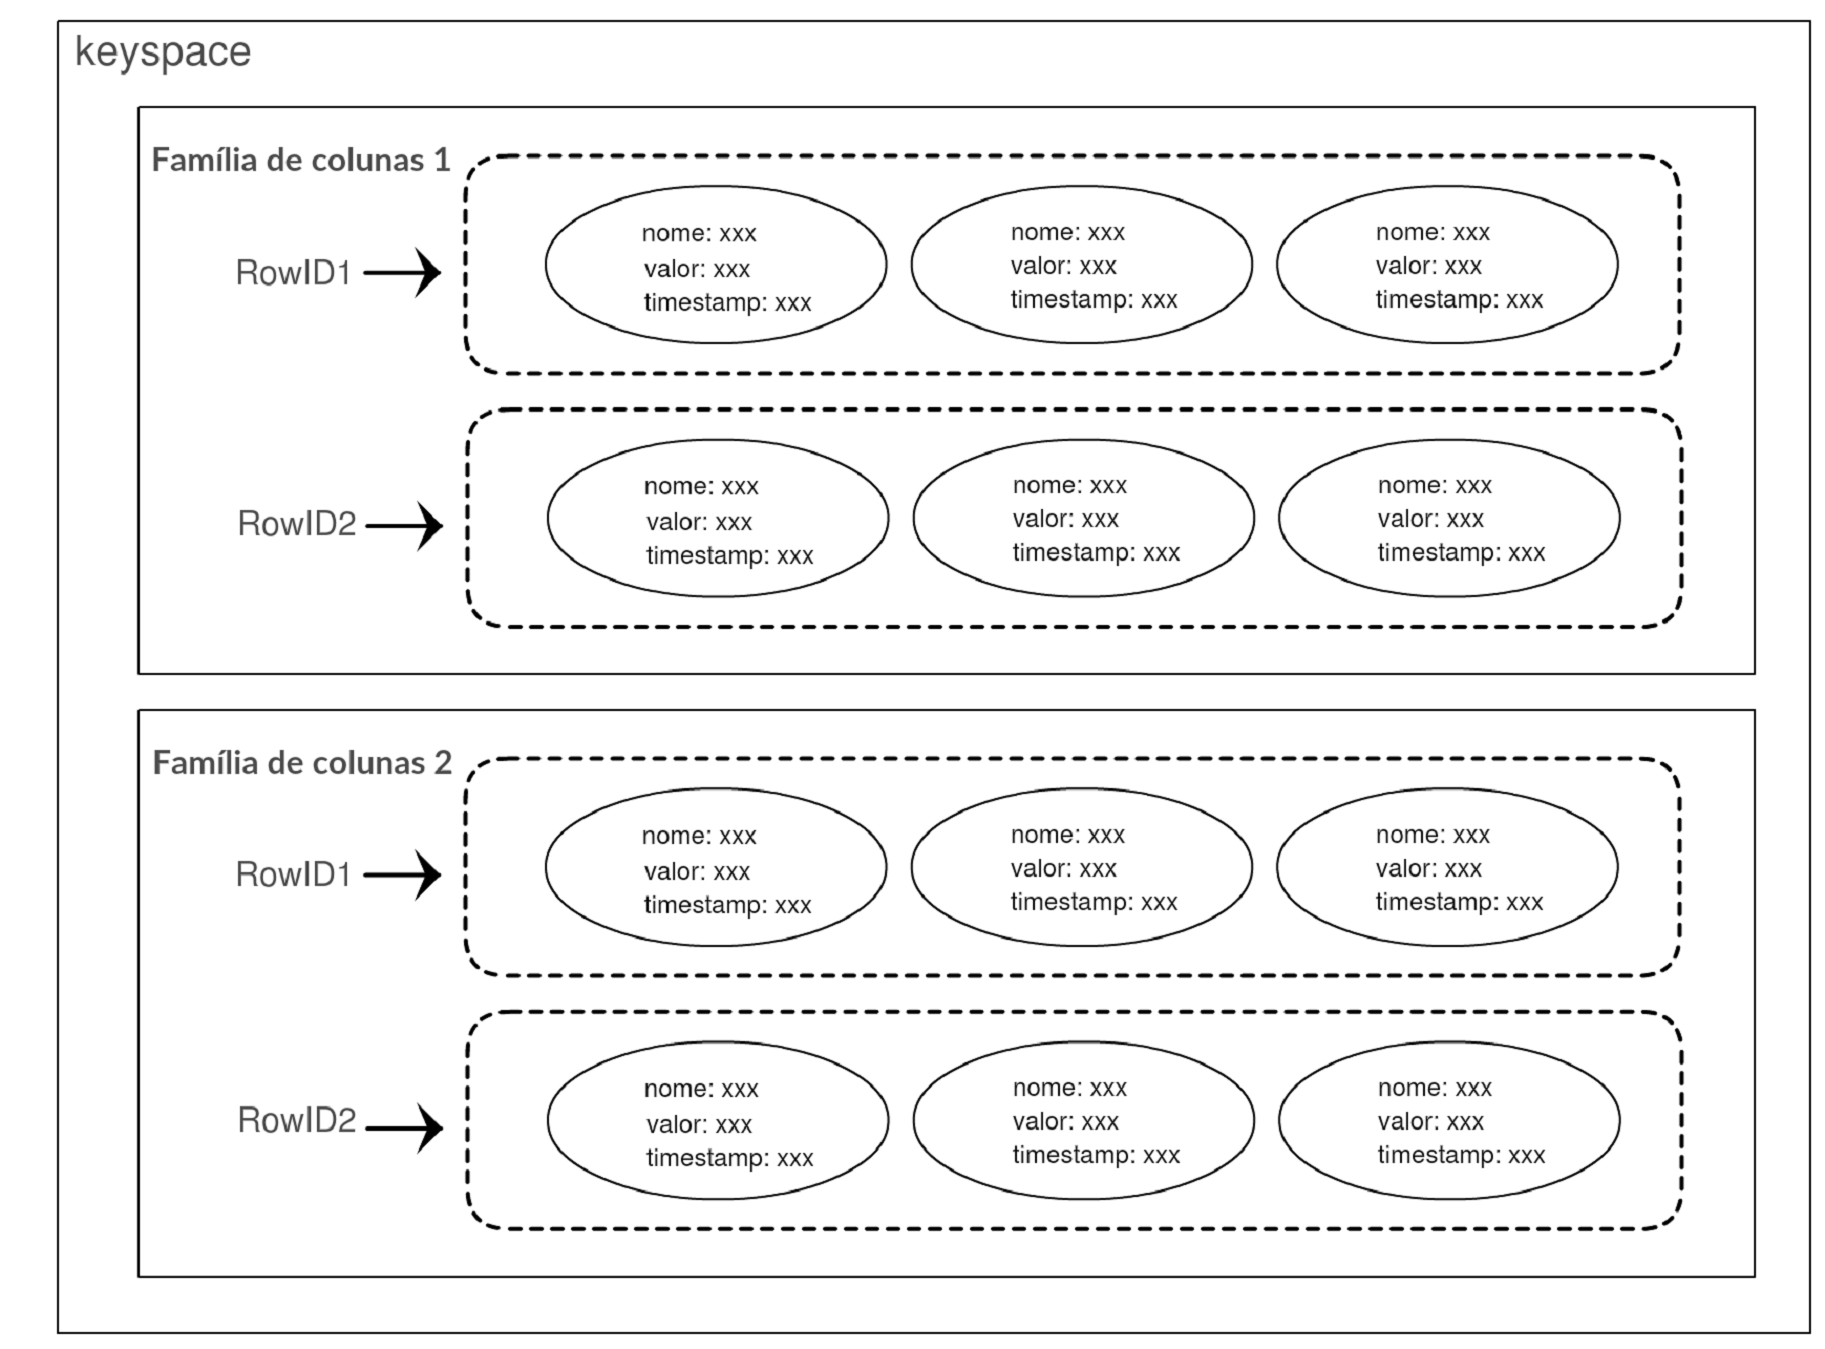
\includegraphics[width=1\textwidth]{figuras/cassandradatamodel.png}
\caption{Modelo de dados do Cassandra. Adaptado de ~\cite{ibmcassandra}}
\label{fig:cassandradm}
\end{figure}

\subsection*{\emph{Keyspace}}
Um \emph{keyspace} define o agrupamento de dados mais externo no Cassandra, podendo ser correspondido a um banco de um SGBD relacional. Um \emph{keyspace} define um nome e uma série de atributos que definem o seu comportamento. 
Atributos do \emph{keyspace} incluem~\cite{cassandraguide}:
\begin{itemize}
\item \textbf{Fator de replicação} diz respeito ao número de nós que armazenarão uma réplica de cada linha de dados. O fator de replicação tem forte influencia no balanço entre performance e consistência do banco de dados.
\item \textbf{Estratégia de replicação} se refere a como as réplicas (ou cópias) de um dado serão posicionados no anel do \emph{cluster}. Diversas estratégias de replicação estão disponíveis no Cassandra.
\item \textbf{Famílias de colunas} pode ser visto como o análogo às tabelas de um modelo relacional, da mesma forma que o \emph{keyspace} é o análogo do banco.  Uma família de colunas é um agrupamento para uma coleção de linhas, onde cada linha contém colunas ordenadas.
\end{itemize}



\subsection*{Colunas e famílias de colunas}
Uma família de colunas (ou tabela) no Cassandra é um mapa multidimensional indexado por uma chave. Essa chave é uma \emph{string} sem restrição de tamanho, mas que em geral varia de 16 a 36 \emph{bytes}. O valor desse mapeamento consiste em uma família de colunas, um agrupamento para uma coleção ordenadas de linhas, que por sua vez é uma coleção ordenada de colunas ~\cite{lakshmancassandra, cassandraguide}.

Uma família de colunas possui dois atributos: um nome e um comparador. O nome identifica a coluna para realização de consultas, enquanto o comparador indica como as colunas serão ordenadas ao serem retornadas em uma consultas, podendo ser \emph{long}, \emph{byte}, UTF8, etc~\cite{cassandraguide}.

O modelo de família de colunas se diferencia do modelo relacional por ser o que é chamado comumente de \emph{livre de esquema} (\emph{schema free}) . É possível realizar a inserção, remoção ou alteração de qualquer coluna ou família de colunas a qualquer momento, ficando as aplicações clientes do banco encarregadas de interpretar e manipular o novo modelo de dados. 

Ao se inserir um novo dado em uma família de colunas do Cassandra são especificados valores para uma ou mais colunas. O conjunto de valores é chamado de linha, e é identificado unicamente por uma chave primária ou chave de linha. Uma linha não precisa possuir dados para todas colunas presentes na família de colunas à que ela pertence, sendo o espaço alocado apenas para as colunas presentes nessa linha. Isso gera tanto uma economia de espaço quanto uma melhora de performance em relação a um banco relacional, que precisa preencher com valores nulos colunas não utilizadas.

Uma coluna é a unidade básica de armazenamento do Cassandra, e é constituída por um nome, um valor e um \emph{timestamp}. Se difere do conceito de colunas de bancos relacionais pois durante a criação do banco não é necessário a criação de colunas, e sim apenas famílias de colunas. A criação de colunas ocorre apenas durante a inserção de dados no banco e suas colunas correspondentes~\cite{cassandraguide}.

\section{Arquitetura}

O Cassandra foi projetado para lidar com grandes massas de dados distribuídas em vários nós sem ponto único de falha, pensado no fato de que tanto um sistema quanto componentes de hardware podem falhar.
Ao contrário de outras soluções de bancos de dados distribuídos, sejam elas relacionais ou modelos mais novos como o \emph{Google Bigtable}, em que os nós são definidos como mestres e escravos (\emph{master} e \emph{slave}), a arquitetura Cassandra combate o problema de falhas ao empregar uma distribuição par-a-par (\emph{peer-to-peer}) entre nós estruturalmente idênticos, com dados distribuídos entre todos os nós de um \emph{cluster}~\cite{cassandradocs, cassandraguide}.  

Essa decisão arquitetural de nós atuando de maneira par-a-par tem como objetivo melhorar a disponibilidade e facilidade de escalabilidade do sistema. Na ocasião de um nó ficar indisponível, existe um potencial impacto na vazão de dados do sistema, entretanto isso não causa uma interrupção no serviço. 
Ao mesmo tempo, ao se inserir um novo nó no sistema, é necessário que ele recebe informações sobre a topologia do anel em que está inserido e dados que ele será responsável. Após isso, entretanto, ele pode integrar o anel e receber requisições assim como os outros nós, sem necessidade de configurações complexas~\cite{cassandraguide}.

O Cassandra é um banco de dados particionado em linhas, com cada linha organizada em tabelas com uma chave primária obrigatória. Sua arquitetura permite que qualquer usuário autorizado se conecte a qualquer nó em qualquer \emph{data center} e acesse os dados por meio da linguagem \emph{CQL}, que possui sintaxe próxima a do \emph{SQL}, com abstração de uma tabela com linhas e colunas~\cite{cassandradocs}. 

Requisições de leitura e escrita podem ser enviadas a qualquer nó do \emph{cluster}, devido à característica de homogeneidade entre eles. Ao realizar uma conexão com um cliente, o nó atua como coordenador dessa operação, servindo de ponte entre a aplicação e os nós que possuem o dado requisitado. O coordenador também determina quais nós devem receber a requisição de acordo com a configuração do \emph{cluster}~\cite{cassandradocs}. 

\subsection{Protocolo Gossip}

Cada nó frequentemente troca informações de estado sobre ele mesmo e outros nós do cluster utilizando um  protocolo \emph{gossip}. \emph{Gossip} é um protocolo de comunicação par-a-par em que os nós realizam  troca de informações periódicas sobre o estados eles mesmos e sobre outros nós do \emph{cluster} de que eles tem conhecimento. Seu nome vem do conceito humano de \enquote{fofoca} (\emph{gossip}), uma forma de comunicação em que cada par pode escolher com quem ele deseja trocar informações~\cite{cassandradocs, cassandraguide}. 

Protocolos \emph{gossip} em geral assumem uma rede falha, e são em geral utilizados em sistemas em rede grandes e descentralizados, em geral em mecanismos de replicação em bancos de dados~\cite{cassandraguide}. 

O processo \emph{gossip} executa a cada segundo, e troca mensagens de estado com até três outros nós no \emph{cluster}. Uma mensagem \emph{gossip} tem uma versão associada a ela, de forma que durante sua troca, informações obsoletas são reescritas com o estado mais atual do nó em questão.

Para evitar problemas na comunicação \emph{gossip}, deve-se utilizar uma mesma lista de nós \emph{seed} para todos os nós do \emph{cluster}. Um nó \emph{seed} é aquele que mantem informações sobre todos os nós da rede. Por padrão, um nó lembra outros nós com quem ele tenha trocada informações entre reinícios do sistema, o nó \emph{seed} tem como única função inicializar o processo \emph{gossip} para novos nós que estejam sendo adicionados ao \emph{cluster}~\cite{cassandradocs}.


\subsection{Operações de Leitura e Escrita}

Ao se realizar uma operação de escrita em um nó, a informação é armazenada imediatamente em um \emph{commit log}. O \emph{commit log} é um mecanismo de recuperação de falhas que garante a durabilidade de um banco Cassandra. Uma operação de escrita só terá sucesso se for escrita no \emph{commit log}, garantindo que mesmo que essa operação não seja armazenada em memória, seja possível recuperar seus dados~\cite{cassandraguide}. 

Os dados do \emph{commit log} são então indexados e escritos em uma estrutura em memória RAM chamada \emph{memtable}. Sempre que os objetos armazenados na \emph{memtable} alcançam um limiar definido, seu conteúdo é carregado em disco em um arquivo \emph{SSTable} e uma nova \emph{memtable} é criada~\cite{cassandraguide, cassandradocs}. 

O conceito da \emph{SSTable} surgiu com o \emph{Google Bittable}. Assim que os dados oriundos da \emph{memtable} são armazenados na \emph{SSTable} eles se tornam imutáveis, não podendo ser modificados pela aplicação. Essa operação de escrita é realizada no final do arquivo (\emph{append}), não sendo necessário leituras ou buscas, razão pela qual o Cassandra é recomendável para sistemas com maior demanda para escritas~\cite{cassandraguide, cassandradocs}.

Os arquivos \emph{SSTable} são então particionados e replicados no cluster, o que garante a redundância dos dados. Periodicamente, as \emph{SSTables} são compactadas e dados obsoletos são descartados, além disso a consistencia do \emph{cluster} é mantida por meio de mecanismos de reparo~\cite{cassandraguide, cassandradocs}. As operações descritas estão esquematizadas na figura \ref{fig:cassandrawriteop}.

\begin{figure}[!htb]
\centering
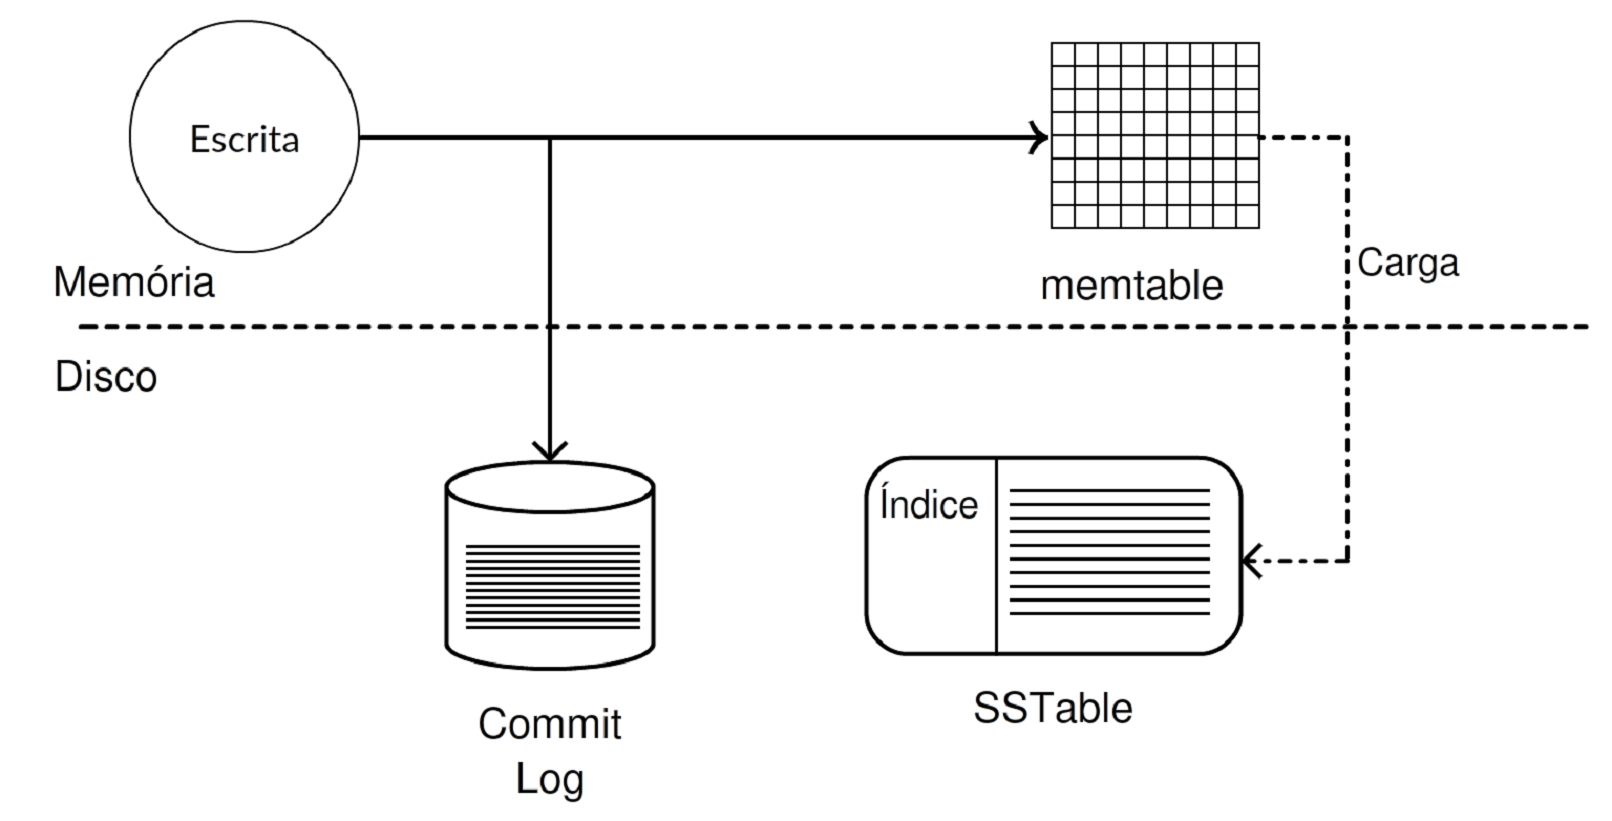
\includegraphics[width=1\textwidth]{figuras/cassandrawriteop.png}
\caption{Escrita de dados em um banco Cassandra. Adaptado de ~\cite{cassandradocs}}
\label{fig:cassandrawriteop}
\end{figure}

Ao se realizar uma operação de leitura o Cassandra inicialmente busca a informação solicitada na \emph{memtable}. Caso não seja encontrada, é realizada uma busca na \emph{cache} de linha, uma estrutura em memória que armazena em memória um subconjunto da partição de dados armazenado nas \emph{SSTable}. Se a \emph{cache} de linha não possuir o dado em específico, é realizada uma consulta no \emph{Bloom Filter} associado à \emph{SSTable} em questão~\cite{cassandradocs}. 

Um \emph{Bloom Filter} é um algoritmo de busca não determinístico que testa de forma rápida se um elemento faz parte de um conjunto. É dito não determinístico pois é possível obter falso positivos em uma consulta, mas não falso negativos. Em outras palavras, um \emph{Bloom Filter} garante que um dado não está presente no conjunto, mas se ele indicar que o dado está presente uma consulta deve ser realizada no conjunto para se obter uma confirmação~\cite{cassandraguide}.

Caso o \emph{Bloom Filter} indique que o dado pode estar presente em uma \emph{SSTable} são realizadas algumas operações de busca de índice para encontrar sua localização, e o dado é então retornado na consulta~\cite{cassandradocs}.

\subsection{Distribuição de Dados}
Distribuição e replicação de dados no Cassandra são conceitos que se conectam. Devido ao fato de um \emph{cluster} Cassandra ser uma rede sem hierarquia entre nós, o sistema faz cópias (ou réplicas) dos dados e as distribui entre os nós. Esses dados são organizados por tabelas identificadas por chaves primárias, que determinam em que nó desse \emph{cluster} esse dado será armazenado~\cite{cassandradocs}.

O Cassandra utiliza um sistema de \emph{hashing} consistente, que permite a distribuição de dados no \emph{cluster} de forma a minimizar a reorganização do mesmo quando nós são inseridos ou removidos. O \emph{hashing} consistente particiona os dados baseados em uma chave de partição (\emph{partition key}), que é obtida do primeiro componente da chave primária de cada tabela. Dessa forma, cada nó em um \emph{cluster} é responsável por um intervalo de dados baseado nesse mapeamento~\cite{cassandradocs}.

A partir de sua versão 1.2 o Cassandra permite que a cada nó físico seja atribuído mais de um \emph{token}, que determina a posição desse nó no anel e a porção de dados de que ele é responsável. Esse novo paradigma de distribuição foi chamado de nós virtuais (\emph{virtual nodes} ou \emph{vnodes}).
Nós virtuais permitem que cada nó possua um grande número de pequenos intervalos de partições distribuídos pelo \emph{cluster}~\cite{cassandradocs}.

A figura \ref{fig:vnodes} mostra a distribuição de nós em um anel, comparando uma arquitetura sem nós virtuais com uma utilizando nós virtuais. 

Na primeira parte da figura a cada nó é atribuído um único \emph{token} que representa sua posição no anel. Cada nó armazena dados determinados pelo mapeamento da chave de partição para um valor no intervalo entre o nó anterior e o valor do \emph{token}. Cada nó também possui réplicas de cada linha de outros nós do \emph{cluster}. 

Na segunda parte da figura, nós virtuais são selecionados aleatoriamente e de forma não contígua. A posição de uma linha é determinada pelo mapeamento da chave de partição dentro de vários pequenos intervalos de partição pertencentes a cada nó~\cite{cassandradocs}.


\subsection*{Replicação de Dados}
O Cassandra armazena réplicas de dados em múltiplos nós para garantir confiabilidade e tolerância a falhas. A estratégia de replicação determina em que nós as cópias serão armazenadas. O número de cópias em um \emph{cluster} é chamado fator de replicação. Se um fator de replicação um é utilizado, existe apenas uma copia de cada linha no \emph{cluster}, ou seja, se o nó contendo essa linha cai, a linha não pode ser acessada. Todas as réplicas são igualmente importantes, não existe uma réplica mestre ou primária. Como regra geral, o fator de replicação não deve exceder o número de nós no \emph{cluster}. É possível, porém, aumentar o fator de replicação e inserir o número desejado de nós posteriormente~\cite{cassandradocs}.

Existem duas estratégias de replicação:
\begin{itemize}
\item \textbf{\emph{SimpleStrategy}} é utilizada para um único \emph{data center} e um único \emph{rack}. A primeira réplica de um nó é determinada pelo particionador, e réplicas adicionais são posicionadas nos próximos nós no anel em sentido horário, sem se considerar a topologia do sistema;
 
\item \textbf{\emph{NetworkTopologyStrategy}} deve ser utilizada quando se tem, ou se planeja ter, um \emph{cluster} distribuído em vários \emph{data centers}. Essa estratégia especifica quantas réplicas se deseja em cada \emph{data center}. As réplicas são inseridas em um mesmo \emph{data center} caminhando-se no anel em sentido horário até se alcançar o primeiro nó em outro \emph{rack}. A \emph{NetworkTopologyStrategy} tenta colocar réplicas em \emph{racks} distintos, por entender que nós em um mesmo \emph{rack} frequentemente falham ao mesmo tempo por problemas de energia, resfriamento ou falhas na rede.
\end{itemize}

Estratégias de replicação são definidas por \emph{keyspace} e definidas durante sua criação~\cite{cassandradocs}.

~\begin{figure}[!htb]
\centering
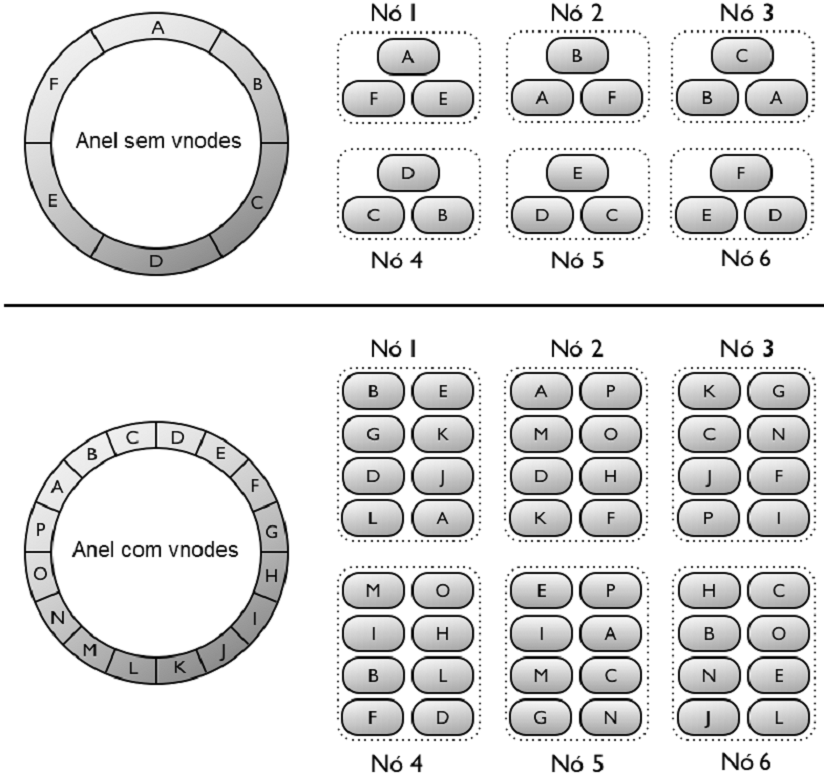
\includegraphics[width=1\textwidth]{figuras/vnodes.png}
\caption{Distribuição de nós em um anel. Adaptado de ~\cite{cassandradocs}}
\label{fig:vnodes}
\end{figure}

\subsection*{Particionadores}
Um particionador determina qual nó irá receber a primeira réplica de um dado e como distribuir outras réplicas entre nós de um \emph{cluster}. Cada linha de dados é unicamente identificada por uma chave primária, que pode ser a mesma que sua chave de partição, mas que também pode incluir outras colunas. Basicamente um particionador é uma função que deriva um \emph{token} a partir de uma chave de primária de uma linha, geralmente por meio de um mapeamento (\emph{hash}). Cada linha de dados é então distribuída no \emph{cluster} de acordo com o valor desse \emph{token}. 

O Cassandra fornece três particionadores, que podem ser definidos no arquivo de configuração principal do Cassandra, o \emph{cassandra.yaml}. São ele:

\begin{itemize}
\item \textbf{\emph{Murmur3Partitioner}} distribui os dados de forma uniforme no \emph{cluster}, de acordo com valores da função \emph{hash} \emph{MurmurHash}, que cria valores de 64 bits com a chave de partição. É o particionador padrão e o recomendável para a maioria dos novos \emph{clusters}, e fornece um desempenho melhor que o do \emph{RandomPartitioner};

\item \textbf{\emph{RandomPartitioner}} também distribui os dados uniformemente no \emph{cluster}, porém com a utilização de uma função \emph{hash} MD5. Essa é uma função criptográfica com um tempo de execução mais longo que a \emph{MurmurHash}. Como o Cassandra não exige um \emph{hash} criptográfico, o particionador \emph{RandomPartioner} reduz o desempenho do Cassandra de 3 a 5 vezes em comparação ao \emph{MurmurPartitioner};

\item \textbf{\emph{ByteOrderedPartitioner}} distribui os nós no \emph{cluster} em ordem alfabética. É utilizado quando se deseja um particionamento ordenado, porém causa problemas de dificuldade de balanceamento de carga, pontos quentes em escritas sequenciais e balanceamento desigual de carga para múltiplas tabelas. É incluído no Cassandra por razões de retrocompatibilidade.
\end{itemize}

Tanto o \emph{MurmurPartitioner} quanto o \emph{RandomPartitioner} utilizam to\emph{tokens} para auxiliar na designação de porções iguais de dados para cada nó e na distribuição de forma uniforme desses dados a partir de todos as tabelas do anel ou de outros agrupamentos, como um \emph{keyspace}.

Ao se selecionar a configuração de quantas réplicas serão armazenadas em cada \emph{data center}, as duas considerações primárias são:

\begin{enumerate}
\item ser capaz de satisfazer leituras locais sem incorrer em latência entre \emph{data centers};

\item cenários de falha.
\end{enumerate}

Os dois modos mais comuns para configurar \emph{clusters} em múltiplos \emph{data centers} são~\cite{cassandradocs}:

\begin{itemize}

\item Duas réplicas por \emph{data center}: essa configuração tolera falhas em nós únicos por grupo de replicação, permitindo ainda leituras locais em um nível de consistência \emph{ONE}.

\item Três réplicas por \emph{data center}: essa configuração tolera tanto a falha de um nó por grupo de replicação em um nível de consistência \emph{LOCAL\_QUORUM} quanto falhas em múltiplos nós com nível de consistência \emph{ONE}

\end{itemize}

Grupos de replicação assimétricos também são possíveis, com cada \emph{data center} adotando a configuração preferível. Já estratégias de replicação são definidas por \emph{keyspace} e definidas durante sua criação~\cite{cassandradocs}.

\subsection*{Níveis de consistência}

Consistência se a quão atuais e sincronizadas todas as réplicas de uma linha de dados do Cassandra está em um dado momento. Operações de reparo automático do Cassandra garantem que todas as réplicas serão eventualmente serão consistentes, porém o tráfego constante de dados entre um sistema largamente distribuído pode levar à inconsistências em algum momento~\cite{cassandradocs}.

Níveis de consistência podem ser configurados para gerenciar o balanço entre disponibilidade de dados e acurácia dos dados. Essa configuração pode se dar dentro de um \emph{cluster}, de um \emph{data center} ou mesmo em operações individuais de leitura e escrita~\cite{cassandradocs}.

Um conceito importante ao se considerar níveis de consistência é o \textbf{quorum}. O nível de \emph{QUORUM} determina o numero de nós que forma um quorum e pode ser calculado pela equação \ref{eq:quorum}~\cite{cassandradocs}.

\begin{equation} \label{eq:quorum}
quorum = ( \frac{Soma Dos Fatores De Replicacao}{2}) + 1
\end{equation}


\subsection*{Consistência de escrita}

A seguir estão listados alguns dos diferentes níveis de consistência de escrita, do mais forte ao mais fraco, sendo o nível \emph{ONE} o nível padrão de consistência~\cite{cassandradocs}:

\begin{itemize}

\item \textbf{\emph{ALL}}: Uma escrita deve ser feita no \emph{commit log} e na \emph{memtable} em todos os nós réplicas em um \emph{cluster} para aquela partição. Fornece a mais alta consistência e mais baixa disponibilidade entre os todos os níveis; 

\item \textbf{\emph{QUORUM}}: Uma escrita deve ser feita no \emph{commit log} e na \emph{memtable} em um quorum de réplicas de nós entre todos os \emph{data center}. Mantém forte consistência porém apresenta certo nível de falha;

\item \textbf{\emph{ONE}}: Uma escrita deve ser feita no \emph{commit log} e na \emph{memtable} de pelo menos um nó. Satisfaz as necessidades da maioria dos usuários, pois não possui exigências rígidas.

\item \textbf{\emph{ANY}}: Garante baixa latência e permite que uma escrita nunca falhe. Fornece a mais alta disponibilidade e a mais baixa consistência

\end{itemize}

\subsection*{Consistência de leitura}

A seguir estão listados alguns dos diferentes níveis de consistência de leitura, do mais forte ao mais fraco, sendo o nível \emph{ONE} o nível padrão de consistência~\cite{cassandradocs}:

\begin{itemize}

\item \textbf{\emph{ALL}}: Retorna um registro depois que todas as réplicas tenham respondido. A operação irá falhar se uma réplica não responder. Fornece a mais alta consistência e mais baixa disponibilidade entre os todos os níveis; 

\item \textbf{\emph{QUORUM}}: Retorna um registro assim que um quorum de réplicas de todos os \emph{data centers} tenham respondido. É utilizado tanto em únicos quanto múltiplos \emph{data centers}, para manter uma forte consistência dentro do \emph{cluster}, desde que seja tolerável certo nível de falha.

\item \textbf{\emph{ONE}}: Retorna uma reposta da réplica mais próxima. Garante a mais alta disponibilidade, desde que seja tolerável uma relativamente alta probabilidade de que um dado antigo seja lido, já que a réplica contatada nem sempre tera a versão mais atual da informação.

\end{itemize}


